\section{Robotics and AI in Ocean Observation}

\begin{wrapfigure}{!h}{2.7in}
  \centering
  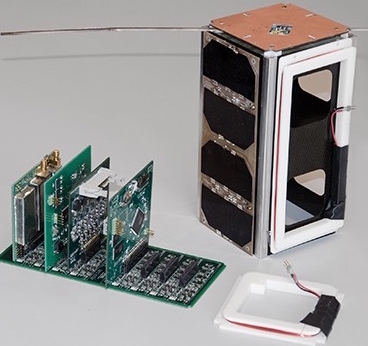
\includegraphics[width=0.4\textwidth]{fig/smallsat.png}
  \caption{\smle's are rapidly moving from technological curiosities
    to operational science platforms adept at earth observing remote
    sensing.}
  \label{fig:sats}
\end{wrapfigure}

The use of robotic assets in ocean observation is relatively
recent. While tethered and immobile 'robots' like moorings have
existed for some time to make in-situ measurements in place, mobile
robots starting with Lagrangian floats, followed by unpowered gliders
\cite{davis02} and now powered AUVs are increasingly making an impact
in scientific exploration. With the recent and ongoing revolution in
miniaturization of sensors, driven in large part by the Smartphone
technologies \cite{yang18}, the impact on marine robotics has been
particularly felt with increasing use of ASVs, many powered by wave or
wind action, and UAVs. ASV's in particular have been adopted widely
for maritime coastal defense \cite{huntsberger11} and monitoring
\cite{johnston17}. What is new is the use of UAVs, from shore and ship
for remotely sensed measurements including ocean color, DiMethyl
Sulfate (DMS), spotting megafauna or measuring the impact of pollution
\cite{dawson17,Ferreira2018,bayirhan19,wei19,pinto20}. Yet awaiting at
the margins of the robotic revolution is a platform, which could
vastly augment the range of applications and observations: the Small
Satellite, a low cost, often student built space vehicle which is
being encouraged as an educational artifact, yet has had little impact
to date on ocean observation \cite{guerra16}.

\smle's are a standardized platform, based on a 10 cm wide cube (1U)
with a mass of up to 1.3 kg with a aluminum based skeleton which can
be integrated with a range of commercial or bespoke instrumentation
(Fig. \ref{fig:sats}). The sizes and payloads can be scaled based on
platform requirements in multiples of this 1U design. The trend to
design and build smaller and more compact payloads, leveraging the
electronics revolution, permits such \smle's to deliver data in
comparable ways to legacy satellite platforms which often take years
to design, build, test and fly; \smle's can often be hoisted within a
year or two at significantly less cost. This has resulted in the use
of the latest hardware (and software) to perform remote sensing
operations hitherto only national or transnational agencies could do,
democratizing space technology. Another distinct advantage that they
offer is a significant reduction in revisit time to provide data over
a fixed region on earth which can often augment data from legacy space
systems. However, significant challenges remain in providing adequate
power, pointing accuracy and payload mass, all of which are part of
ongoing research efforts.

\begin{figure}[!t]
  \centering
  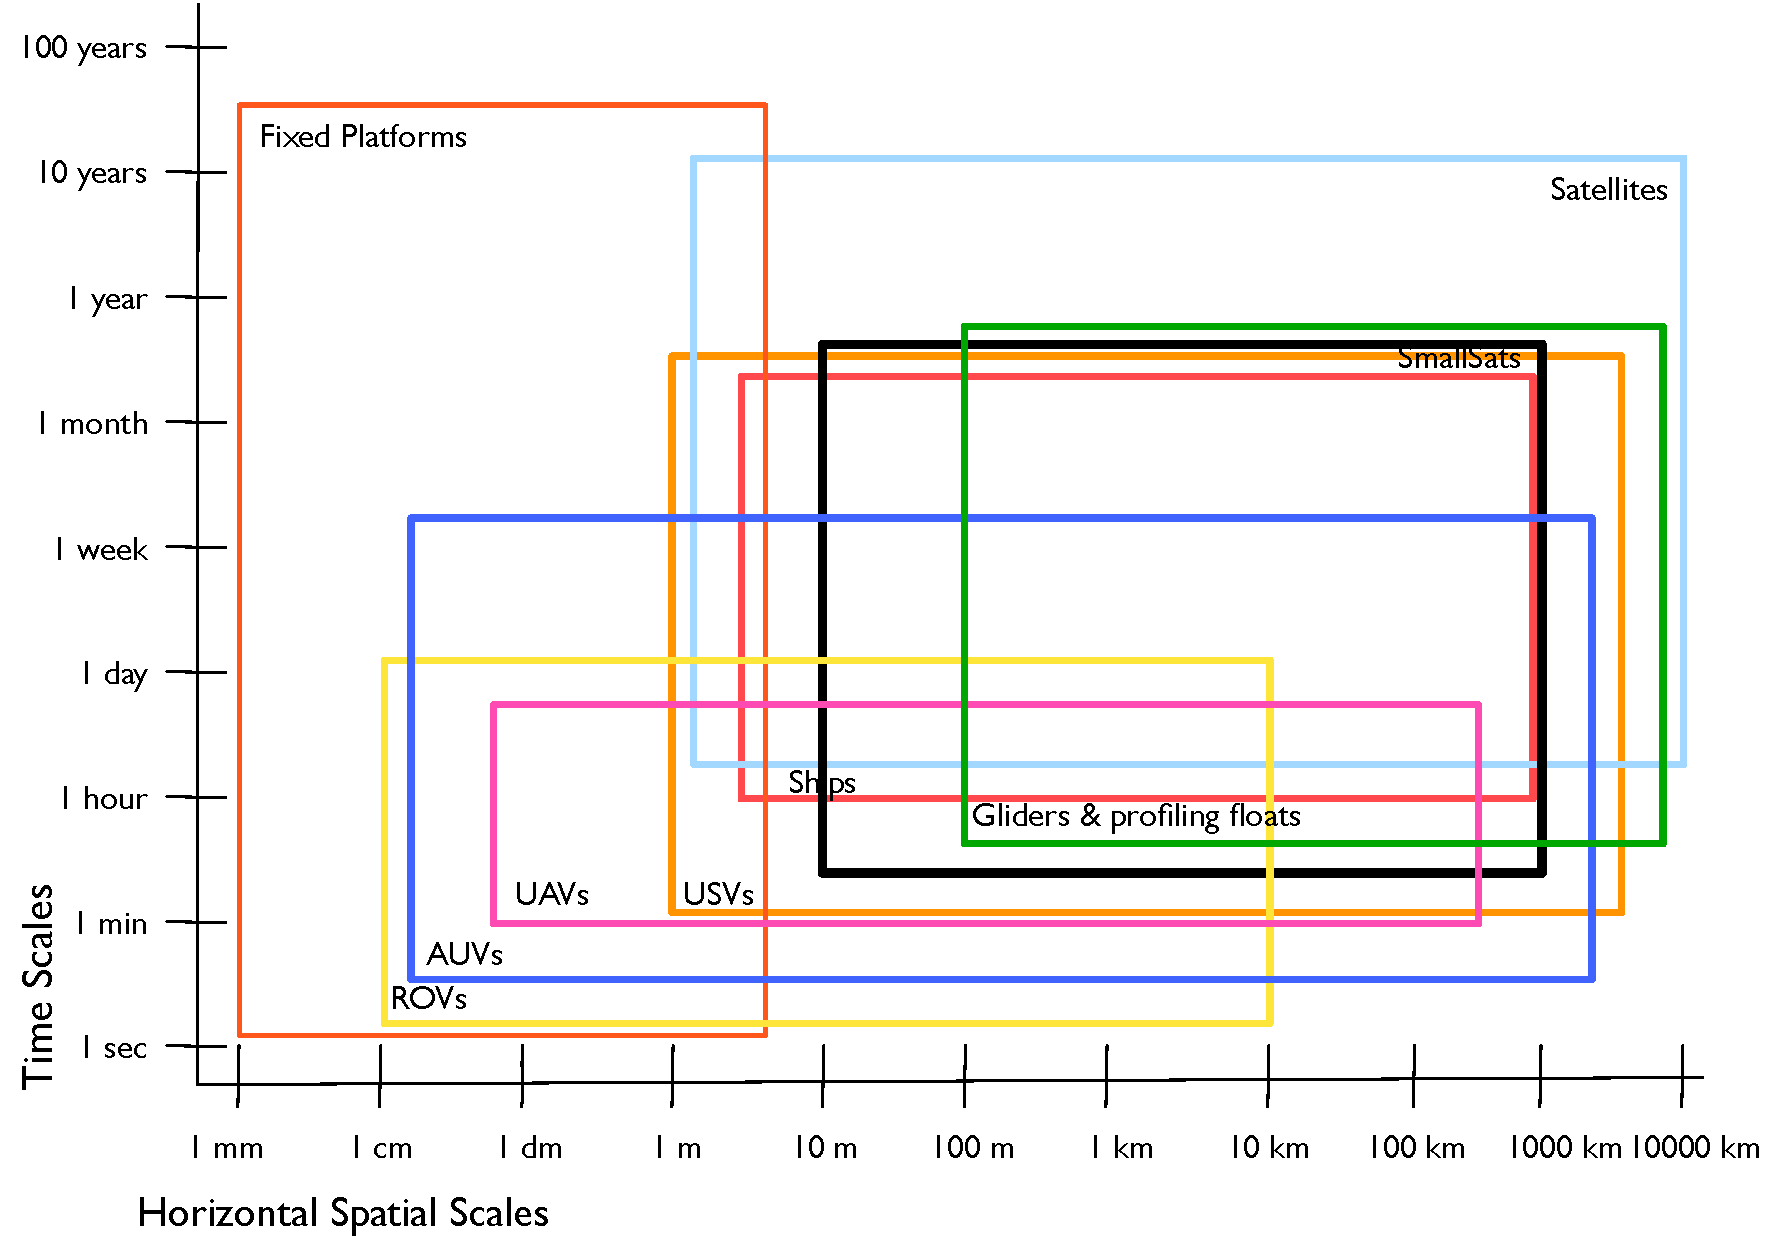
\includegraphics[width=0.7\textwidth]{fig/platform-capabilities.pdf}
  \caption{While \smle's do not occupy a unique position in ocean
    observation, overlapping a range of other assets, their capability
    for controlled observations along institutional lines is a
    harbringer of complementary views of the earths oceans. Figure
    modified from \cite{haury78}.}
  \label{fig:platforms}
\end{figure}

Fig. \ref{fig:platforms} shows how various robotic platforms' spatial
coverage maps into typical persistence in observation. Fixed platforms
such as moorings and buoys for instance, can be displaced a few meters
at most, but can provide observation continuity for decades if
maintained appropriately. Conversely platforms like UAVs can cover
vast distances, but their energy requirement constraints them to
operate at most a few hours. Powered AUVs with the latest battery
chemistry can operate up to a week while covering hundreds of
kilometers; gliders, can do better at slower speeds and cover larger
distances, yet their payload is constrained by onboard battery. 


\begin{wrapfigure}{!h}{2.7in}
  \centering
  \subfigure[]{\label{fig:platforms1}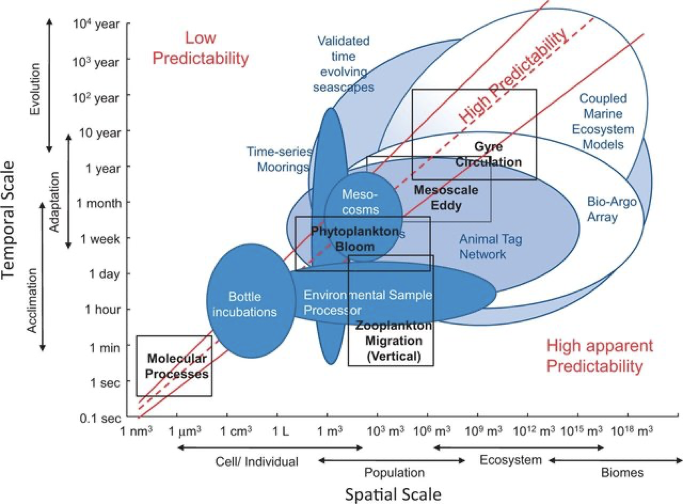
\includegraphics[width=0.5\textwidth]{fig/bio-processes.png}}
  \subfigure[]{\label{fig:platforms2}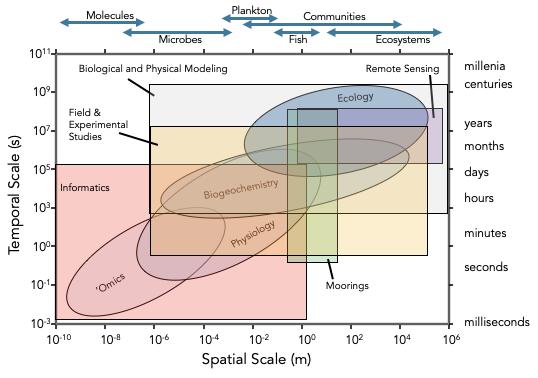
\includegraphics[width=0.5\textwidth]{fig/spatio-temporal.png}}
  \caption{\kc{Note these are placeholders from Ajit. I think these
      two figures can contribute to shaping the narrative quite a bit.}}
\end{wrapfigure}

While robotic platforms are critical to ocean observation, the
ultimate goal is to generate data from sensors which can be collated
and fused to provide \emph{information} in usable ways, to understand
causality, structure and process for the study of the upper
water-column. \kc{Need something meaty here to show what we mean by
  'fusing'} 

\subsection{AI and its application to Ocean Observation}

Much has been made of the revolution in data science and Machine
Learning (ML) in recent times, the impact of these sub-fields of
Artificial Intelligence and AI as a whole has been glancing. By 'AI'
we mean here the original notion of using logical formalisms tied to
computational decision making. At its heart lies the notion of
computational search where selection of possible outcomes of a
decision is informed either by a model, a heuristic or some principled
approach, so the outcome is deterministic if contextual. However the
conflating of data science and ML with 'AI' has added more confusion
than provided clarity in what researchers need to or ought to work on
to progress the science.

To understand causality of process function in the water-column, data
(e.g. temperature, salinity, oxygen, fluorescence, pH, \ldots) needs
to be collected and time-series need to be compiled over a period of
time to encompass tidal, seasonal and climatic variability. These are
typically adduced to generate some form of causal explanation for
human understanding that is at the heart of what is needed to create
knowledge about a changing planet. Where ML has provided insights in
the ocean sciences therefore has been on shore-side computation using
vast computing and data resources, post-facto to the actual
observational data collected \kc{Need citations}. A different effort
underway has been to use \emph{offline} neural network learned models
to actually impact \emph{online} observation making by a mobile robot
\cite{saad20} \kc{Add Yogi's mapping by surprise material
  here}. Separately, statistical methods in information theory, have
been used with far more practical outcomes to how a robot actually
samples in the water column
\cite{jdas13,das15,fossum18,fossum18b}. Newer methods in Statistical
ML applied to ocean sampling has also advanced the applicability in
where and when to sample in dynamic regions with discernable features
such as fronts and plumes \cite{fossum21}.

Where there has been markedly more effort and success, has been in the
\emph{control} of vehicles mostly on the surface or underwater, where
more systematic methods in AI have been brought to bear. Control of
such robots
\cite{benjamin2010,das11,das11b,olaya12,graham12,fossum18,fossum18b,pinto20}
including efforts for systematic coordination of aerial and underwater
vehicles \cite{Ferreira2018} as also some significant efforts in
mapping benthic communities \cite{johnson17} has been the hallmark of
efforts by technologists, to date.


% Lagrangian floats initiated the development of untethered
% devices, initially to measure sub-surface currents in the ocean via
% ocean acoustics. By being neutrally buoyant, these Lagrangian devices
% could then float with the current and periodically reach the surface,
% by changing their buoyancy, to communicate data and then return
% subsurface. Variations of float designs evolved into the design of an
% underwater glider with wings, a buoyancy engine and a method to shift
% weights to deal with pitch and yaw motion; this work was led by Doug
% Webb and Russ Davis \cite{davis02} motivated by a seminal article by
% Hank Stommel who imagined how glider fleets could traverse the worlds
% oceans over months making measurements while surveying vast stretches
% of the ocean \cite{stomme89}. While propelled vehicles were
% experimented upon as engineering artifacts \cite{blidberg01}, glider
% development for scientific exploration provided a filip to the use of
% AUVs.


% While research related to atmospheric phenomenon has long
% leveraged technology including remote sensing satellites, generating
% ocean measurements has been substantially more
% challenging. Observations from satellites cannot penetrate more than a
% few centimeters from the surface, sunlight does not permeate beyond
% the photic zone and crushing pressure requires instrumentation to be
% simple to operate yet robust to be able to survive. Terrestrial
% techniques in robot sensing and perception typically do not translate
% into making oceanographic measurements.

% The advent of lagrangian floats initiated the development of
% untethered devices, initially to measure sub-surface currents in the
% ocean via ocean acoustics. By being neutrally buoyant, these
% Lagrangian devices could then float with the current and periodically
% reach the surface, by changing their buoyancy, to communicate data and
% then return subsurface. Variations of float designs evolved into the
% design of an underwater glider with wings, a buoyancy engine and a
% method to shift weights to deal with pitch and yaw motion; this work
% was led by Doug Webb and Russ Davis \cite{davis02} motivated by a
% seminal article by Hank Stommel who imagined how glider fleets could
% traverse the worlds oceans over months making measurements while
% surveying vast stretches of the ocean \cite{stomme89}. While propelled
% vehicles were experimented upon as engineering artifacts
% \cite{blidberg01}, glider development for scientific exploration
% provided a filip to the use of AUVs.

% While we are still at early stages of development of such platforms,
% with sufficient computational and energy resources, yet their adoption
% for science has proven to be surprisingly quick. Early adoption of
% such 'robotic' vehicles from floats and gliders were traditionally
% driven by the study of ocean physics (the study of currents,
% acoustics, wind and the impact of bathymetry and surface
% topology). More recent efforts however, have seeped into ocean biology
% with the use of physical measurements as a means to understand the
% presence and community structure of organisms from the micro to the
% macro and highly inter-disciplinary studies of ecology of the coastal
% as well as the deep ocean, thereby merging observations in physical
% and bio-geochemical oceanography as a means to study ecosystems,
% typically at the meso-scale. The emergence of ocean remote sensing has
% also provided an inordinate amount of information about the upper
% ocean, in ways that have previously been challenging to obtain,
% especially at large spatio-temporal scales. Together, this has
% resulted in the possibility of defining a new paradigm of ocean
% observation and consequently of marine robotics. While the latter has
% also had a profound impact from commercial Oil and Gas exploration
% (especially with the advancement of tethered remotely operated
% vehicles) and maritime defence, as also the use of \emph{immobile}
% Eulerian 'robots' such as moored surface and sub-surface buoys, our
% focus in this work is geared towards civilian oceanographic
% observations using mobile platforms.


% Trace the advent of scientific instrumentation which morphed into
% floats, into gliders and powered AUVs.

% \begin{enumerate} 

%   % \item articulate the various 'robotic' vehicles, mobile and
%   %   immobile. Keep this general, so even a buoy is a robotic sensing
%   %   platform

%   \item how an ensemble of vehicles can extend the “reach" of the
%     human senses onboard the ship and perhaps even from shore with
%     high bandwidth comms -- extend the above to not just water-column,
%     but benthic work (where I know very little)

%   \item Show the figure of which robotic assets are viable for what
%     kinds of observation. Overlay bio-physical processes which are
%     appropriate and discuss at length why these assets suit those
%     specific observations.

%   \item Articulate how robots have 'extended the human senses' from
%     ship and shore to provide new ways of observing the ocean

%   \item In brief -- examples of Machine Learning and other forms of AI
%     which can help and how (see below). Machine Learning offline or
%     even inline in the perspective of “discovery"

%   \item How systematic observation, as against point measurements
%     (i.e. dipping a rosette) and using extrapolation, can help. What
%     kinds of signals are being missed

%   \item Harshness of the environment and operational issues of being
%     at sea for sustained presence

% \end{enumerate}
